\documentclass[a4paper,12pt]{article}

\usepackage{graphicx}
\usepackage{hyperref}
\usepackage{amssymb}
\usepackage{amsmath}

\title{Reasoning \& Logic (CSE1300) --- Summary}
\author{Dany Sluijk}
\date{September/October 2018}

\makeindex

\begin{document}
\maketitle
\begin{center}
	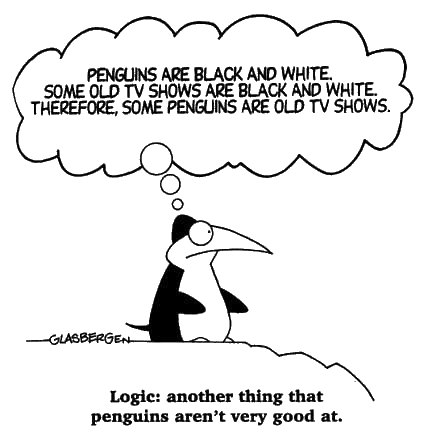
\includegraphics[height=9cm]{./intro}
\end{center}
\begin{abstract}
	This document contains a summary of the Reasoning \& Logic course given
	in the first year of Computer Science and Engineering.
	This is \emph{not} a definitive guide, and might contain errors.
	Please send an email to \href{mailto:dany@atlasdev.nl}{``dany@atlasdev.nl''}.
	A lot of information in this book is taken with fair use from the
	\href{https://textbooks.open.tudelft.nl/index.php/textbooks/catalog/book/13}{``Delftse Foundations of Computation''}
	book created by Stefan Hugtenburg and Neil Yorke-Smith.
	This summary is distributed under the same
	\href{https://creativecommons.org/licenses/by-nc-sa/4.0/}{CC BY-NC-SA 4.0} license.
\end{abstract}

\newpage
\tableofcontents

\section{Propositional Logic}

Propositional logic is about arguments.
An argument contains two things:

\begin{itemize}
	\item
	      One or more premises.
	\item
	      One conclusion.
\end{itemize}

Both of these things must be propositions.
This means they must evaluate to either true ({\bf 1}) or false ({\bf 0}).
Take the following example:

\begin{table}[h]
	\centering
	\begin{tabular}{l}
		All humans are mortal \\
		Socrates is human     \\
		\hline
		$\therefore$ Socrates is mortal
	\end{tabular}
	\caption{An example of an argument in English}
\end{table}

In this example a premise ``All humans are mortal'' is given.
This is something which can be either true or false.
Given that both premises are true, we must accept the conclusion to also be true.
In this case that means Socrates is a mortal.
Propositional logic is not a one-size-fit-all solution.
It does not have {\bf quantifiers}, which means you cannot specify an amount of something.
Propositional statements are generally not in english.
The are replaces with {\bf propositional variables} like \(p\), \(q\) and \(r\).

\subsection{Valid $\neq$ Sound}
There is a difference in {\bf sound} and {\bf valid} arguments.
A {\bf valid} argument is an argument which is `syntactically' valid.
This means that the argument holds if all permises are true, but it does not mean the permises hold up.
When the arguments hold up in the real world, then the argument is also {\bf sound}.
The given example is both valid as well as sound.
If you change both occurances of `mortal' to `immortal'
then the example is still valid, but no longer sound as the argument no longer holds up in the real world.

\subsection{Logical connectives}
{\bf Logical connectives} or {\bf logical operators} is the `glue' between propositions.
A list of possible logical connectives are shown in table \ref{tab:logicalConnectives}.
Logical connectives can be used to compare or combine multiple propositional variables.
Take for example the following formula: \(q \land p\).
This takes two propositional variables \(p\) and \(q\) and compares that.
This returns another boolean, namely true when both \(p\) and \(q\) are true, or false in every other case.
Using this knowledge you can create something called a {\bf compound proposition}.
This means it combines multiple proposition to a single, larger one.
An example of a compound proposition is \((q \land p) \lor \neg r\).
Both \(q \land p\) and \(\neg r\) are propositions, and combining gives a new one.
If you execlude the parenthesis then the formula is parsed from left to right.
So \(q \land p \land r\) is equal to \((q \land p) \land r\) but not to \(q \land (p \land r)\).

\begin{table}[h]
	\centering
	\begin{tabular}{c | l | l}
		Symbol     & Name         & Effect                                                \\
		\hline
		$\land$    & conjunction  & True when both propositions are true                  \\
		$\lor$     & disjunction  & True when one or both propositions are true           \\
		$\oplus$   & exclusive or & True when one of the propositions is true             \\
		$\neg$     & negation     & True when the proposition is false                    \\
		$\implies$ & implication  & True if both sides are true or the left side is false \\
		$\iff$     & iff          & True if both sides are true                           \\
	\end{tabular}
	\caption{A list of logical connectives}
	\label{tab:logicalConnectives}
\end{table}

\subsection{Logical equivalence}
If you want to check if two propositions are equivalent
(e.g. have the same value all the time), then you can use a {\bf truth table}.
A truth table is an table with all possible outcomes of a proposition.
If two propositions have the outcome in the truth table then the two propositions are equivalent.
take this truth table for example:

\begin{table}[h]
	\centering
	\begin{tabular}{c | c | c | c}
		\(q\) & \(p\) & \(q \land p\) & \(\neg(\neg q \lor \neg p)\) \\
		\hline
		0     & 0     & 0             & 0                            \\
		0     & 1     & 0             & 0                            \\
		1     & 0     & 0             & 0                            \\
		1     & 1     & 1             & 1                            \\
	\end{tabular}
\end{table}

As you can see, the two statements have the same values in the truth table, and are logically equivalent.

\subsection{Sufficient or Necessary}
Given is the following implication \(p \implies q\).
\(p\) is in this statement the {\bf hypothesis}, and \(q\) is the {\bf conclusion}.
If the hypothesis is true then it's sufficient to say the conclusion is also true.
If the conclusion is true then it's necessary to say the hypothesis is also true.
It's impossible for the conclusion to be false if the hypothesis is true.
But when the hypothesis is false then the conclusion can be both true and false.
So if the hypothesis is false then you can say that the statement holds.

\subsection{Contrapositive, Converse and Inverse}
Every implication has a contrapositive, converse and a inverse.
They can, but don't have to be logically equivalent.
Given the implication `If this is Tuesday, then we are in Belgium' or in logic form \(p \implies q\)
we can get the contrapositive, converse and inverse of it.
The {\bf contrapositive} is \(\neg q \implies \neg p\), so `If we aren't in Belgium, then this isn't Tuesday'.
The {\bf converse} is \(q \implies p\), so `If we are in Belgium, then this is Tuesday'.
The {\bf inverse } is \(\neg p \implies \neg q\), so `If this isn't Tuesday, then we aren't in Belgium'.

\subsection{Tautology, Contradiction and Contingency}
There are more categories where propositions can fit in. These three are one of those.
A tautology is a proposition which always evaluate to true. An example is the proposition \(q \lor \neg q\).
A contradiction is the opposite, it'll always evaluate to false. An example is \(q \land \neg q\).
A contingency is every thing else, which can be true or false. For example \(q\).

\begin{table}[h]
	\centering
	\begin{tabular}{c | c | c | c}
		\(q\) & \(q \lor \neg q\) & \(q \land \neg q\) & \(q\) \\
		\hline
		0     & 1                 & 0                  & 0     \\
		0     & 1                 & 0                  & 0     \\
		1     & 1                 & 0                  & 1     \\
		1     & 1                 & 0                  & 1     \\
	\end{tabular}
\end{table}
\end{document}